%adobe reader fix
\pdfminorversion=4

\documentclass[final]{beamer}

%set image/logo options
% Rice
\def\RightLogoWidth{0.18}
\def\RightLogoPaddingTop{0.25cm}
\def\RightLogoPaddingBottom{0.5cm}
\def\RightLogo{../logos/RiceLogo_TMCMYK300DPI.jpg}
% SunPy
\def\LeftLogoWidth{0.06}
\def\LeftLogoPaddingTop{0.25cm}
\def\LeftLogoPaddingBottom{0.25cm}
\def\LeftLogo{../logos/sunpy_powered_logo.png}
% Title and author(s) block
\def\TitleWidth{0.7}
% GitHub
\def\GitHubLogoWidth{0.014\paperwidth}
\def\GitHubLogo{../logos/GitHub-Mark-120px-plus.png}
\def\GitHubUser{wtbarnes}
% Affiliation in footer
\def\AffiliationFooter{Department of Physics and Astronomy - Rice University - Houston, TX USA}
% Email
\def\EmailAddressFooter{will.t.barnes@rice.edu}

%set theme
\mode<presentation>
{
\usetheme{I6dv_custom}
}
\setbeamertemplate{caption}[numbered]

%Include packages
\usepackage{soul,color,verbatim}
\usepackage{type1cm}
\usepackage{calc}
%\usepackage{times,mathptmx}
\usepackage{amsmath,amsthm,amssymb,latexsym}
\usepackage{empheq}
\usepackage{graphicx}
\usepackage{epstopdf}
\usepackage[numbers]{natbib}
\usepackage{multicol}
\usepackage{subfigure}

\usepackage[english]{babel}
%\usepackage[latin1]{inputenc}
\usepackage{tikz}
%setup beamerposter package
\usepackage[orientation=portrait,size=custom,width=91.44,height=121.92,scale=1.0]{beamer/beamerposter/beamerposter}

%tikz configuration

%custom commands go here
\newcommand{\ang}{\AA~} %alias angstrom
\setbeamerfont{caption}{size=\footnotesize} %make caption size small
\DeclareMathOperator*{\argmax}{\arg\!\max}

%Set author and title
\title[AR Timelag Analysis]{Timelag Analysis of Global Hydrodynamic Simulations of Active Regions in the Solar Corona}
\author[Barnes \& Bradshaw]{Will T. Barnes \& Stephen J. Bradshaw}
\institute[Rice University]{Department of Physics and Astronomy, Rice University\\
                            Rice Data Science Conference, 9-10 October 2017}
\date{9-10 October, 2017}

%start poster
%everything goes in one frame
\begin{document}
\begin{frame}
  %start columns environment to slice up the page horizontally
  \begin{columns}[T]
  \hfill
  %%
  %%first column
  \begin{column}{0.49\linewidth}
    %
    %introduction
    \begin{block}{The Coronal Heating Problem}
        \begin{itemize}
        \item Fundamental question: \alert{what is the frequency of energy release in the cores of active regions (ARs)?}
        \item Define heating frequency in terms of $t_N$, the time between successive heating events on a \textit{single strand}, and $\tau_{cool}$, a typical loop cooling time,
        \begin{itemize}
            \item Low-frequency heating: $t_N>\tau_{cool}$ (i.e. approaches single nanoflare case), 
            \item High-frequency heating: $t_N<\tau_{cool}$ (i.e. approaches steady heating case), 
        \end{itemize}
        \item Using a robust forward modeling framework and emission measure diagnostics, we address two primary questions:
        \begin{enumerate}
            \item \alert{What are the observational signatures of nanoflares of varying frequency?}
            \item \alert{Can these signatures be observed and be used to constrain the heating frequency in AR cores?}
        \end{enumerate}
        \end{itemize}
        \begin{figure}
            \centering
            \begin{columns}
                \column{0.7\columnwidth}
                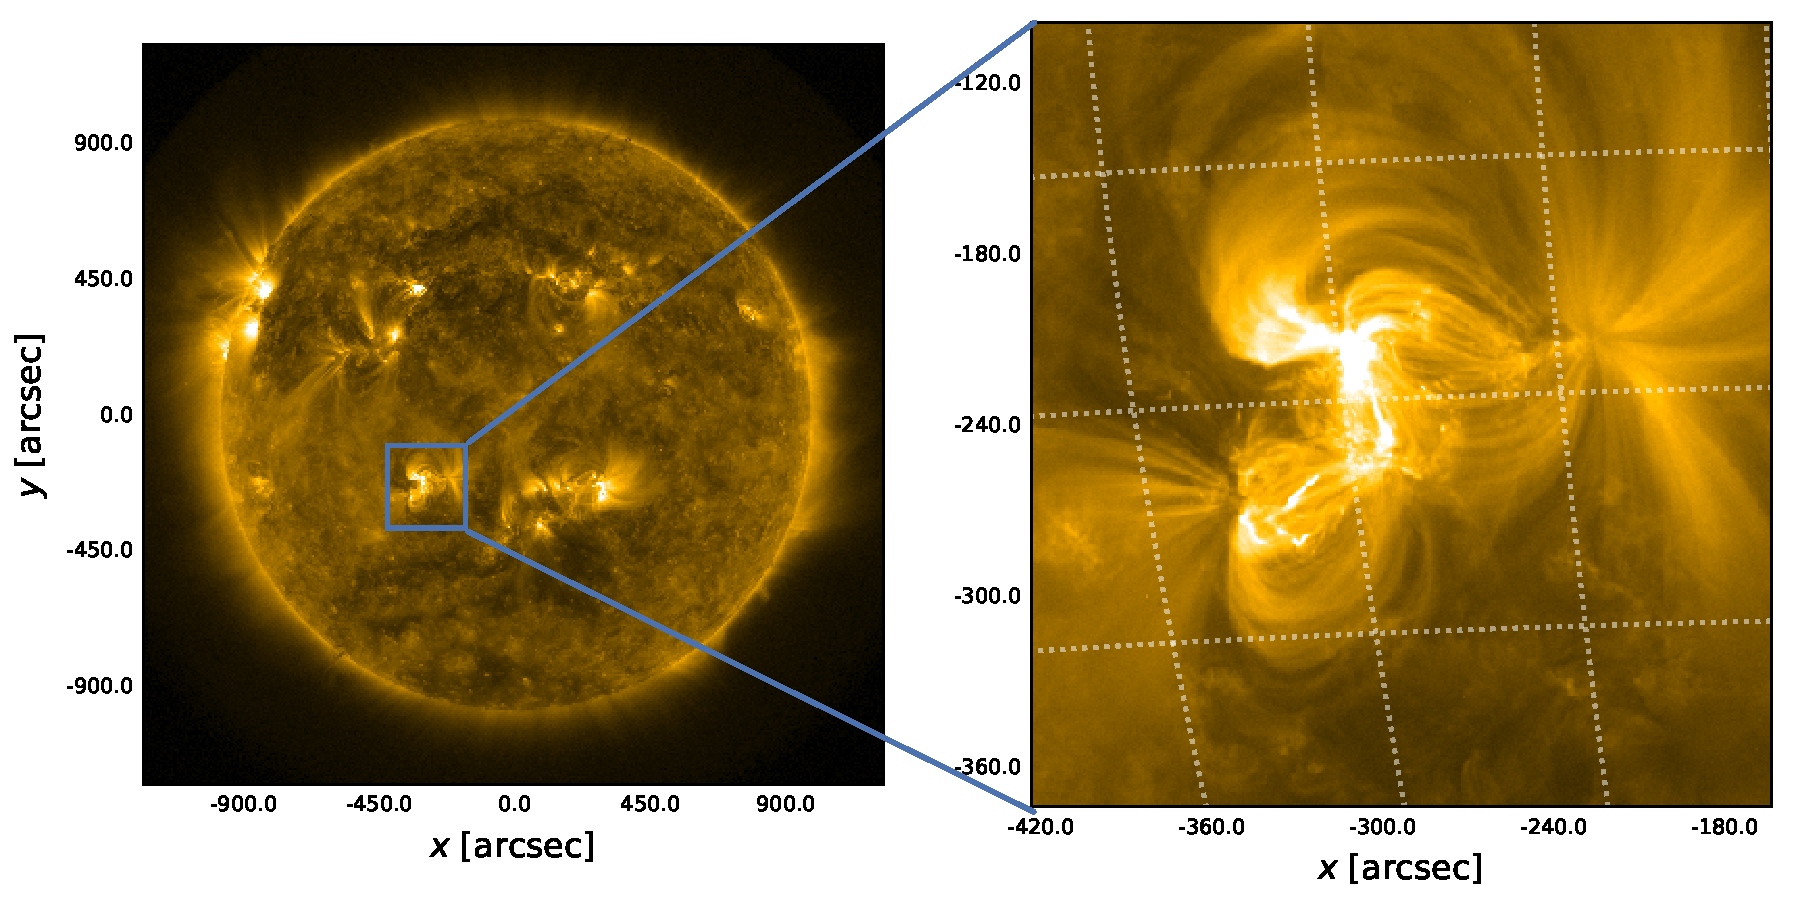
\includegraphics[width=\columnwidth]{figures/fulldisk_plus_zoom_171.pdf}
                \column{0.29\columnwidth}
                \caption{\textbf{Left:} The full solar disk as imaged by the Atmospheric Imaging Assembly (AIA) instrument on the Solar Dynamics Observatory (SDO) on 12 February 2011 15:30:37 UTC. Shown here is the 171 $\mathrm{\mathring{A}}$ EUV channel which images plasma around 1 MK. \textbf{Right:} A zoomed-in view of active region (AR) NOAA 1158. Note the clearly visible loop structures where the plasma is confined along the strong magnetic field and the roughly dipole-like structure. ARs are areas of intense magnetic activity where coronal plasma can be heated in excess of 10 MK.}
            \end{columns}
        \end{figure}
    \end{block}
    %
    %% loop hydrodynamics
    %% Talk about hydro models
    \begin{block}{Loop Hydrodynamics}
    \begin{itemize}
        \item Because the solar corona is a \alert{low-beta} plasma, we can treat the corona as an ensemble of one-dimensional strands and solve hydrodynamic equations along these structures, e.g. like water confined to flow through a pipe 
        \item Use a ``0D'' two-fluid hydrodynamic code \citep{klimchuk_highly_2008,cargill_enthalpy-based_2012,barnes_inference_2016} to efficiently compute time-dependent solutions for \alert{many} loops,
        \begin{eqnarray}
            \frac{dp_e}{dt} &=& \frac{\gamma - 1}{L}(\psi_{TR} - (\mathcal{R}_{TR} + \mathcal{R}_C)) + k_Bn\nu_{ei}(T_i - T_e) + (\gamma - 1)Q_e \\
            \frac{dp_i}{dt} &=& -\frac{\gamma - 1}{L}\psi_{TR} + k_Bn\nu_{ei}(T_e - T_i) + (\gamma - 1)Q_i \\
            \frac{dn}{dt} &=& \frac{c_2(\gamma - 1)}{c_3\gamma Lk_BT_e}(\psi_{TR} - F_{ce,0} - \mathcal{R}_{TR})
        \end{eqnarray}
        \item Efficient, well-benchmarked model \citep[see][]{cargill_enthalpy-based_2012-1,barnes_inference_2016} that includes enthalpy flux, thermal conduction ($F_{ce,0}$), radiation ($\mathcal{R}_{TR},\mathcal{R}_C$), collisions between electrons and ions ($\nu_{ei}$)
        \item Note that the heating term ($Q_e,Q_i$) is time-dependent and a \alert{free parameter}--adjust the frequency and magnitude of the heating and compare to observations in order to assess the viability of different heating models
    \end{itemize}
    \end{block}
    %
    % forward modeling
    %% Describe synthesizAR code, maybe a diagram?
    \begin{block}{Forward Modeling Emission from Active Region Cores}
        % forward modeling details here
        % show HMI map with lines
        % equation for intensity calculation
        % discuss steps
    \begin{columns}[T]
        \begin{column}{0.49\columnwidth}
            \begin{figure}
                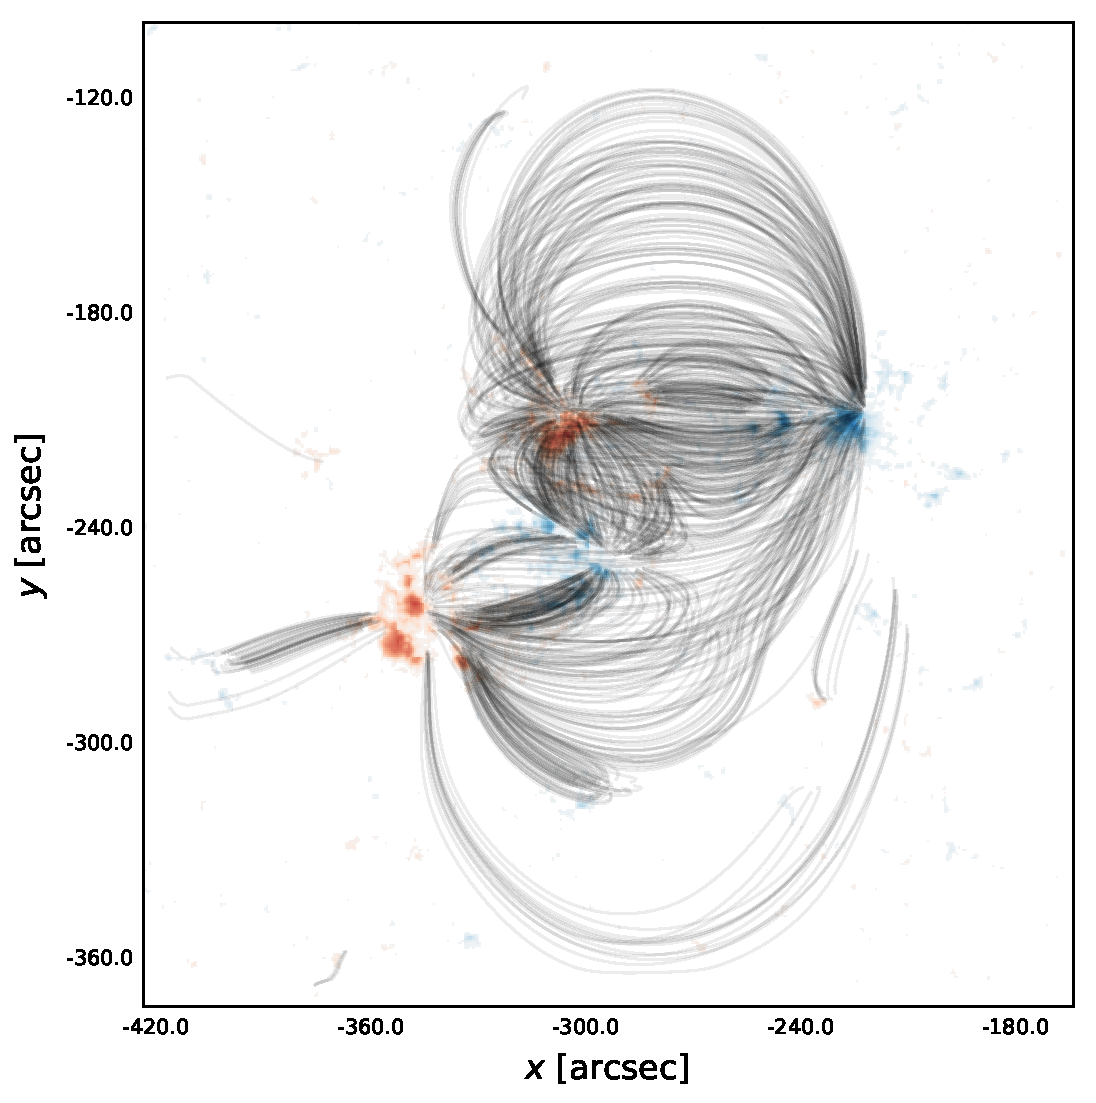
\includegraphics[width=\columnwidth]{figures/hmi_map_with_strands.pdf}
                \caption{...}
                \label{fig:hmi_map}
            \end{figure}
            \begin{figure}
                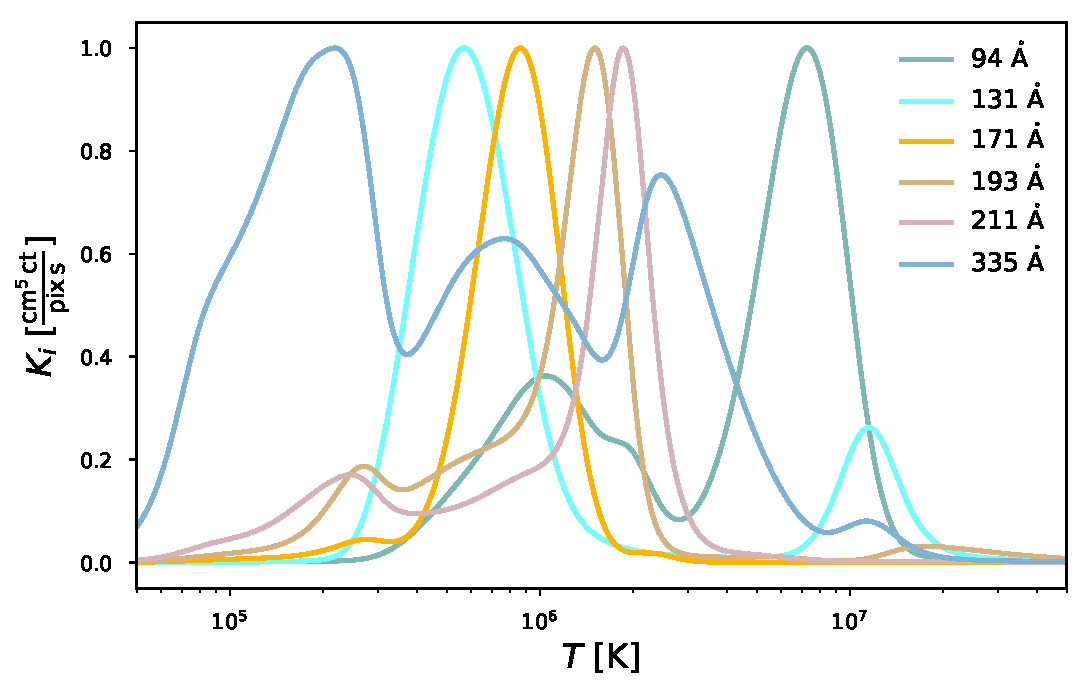
\includegraphics[width=\columnwidth]{figures/aia_response_functions.pdf}
                \caption{...}
                \label{fig:response_functions}
            \end{figure}
        \end{column}
        \begin{column}{0.49\columnwidth}
        \end{column}
    \end{columns}
    \end{block}
    %
    %
    % AIA intensity
    %% AIA intensity maps for a given heating model 
    \begin{block}{Synthesizing AIA Intensities}
        \vspace{-2ex}
        \begin{figure}
            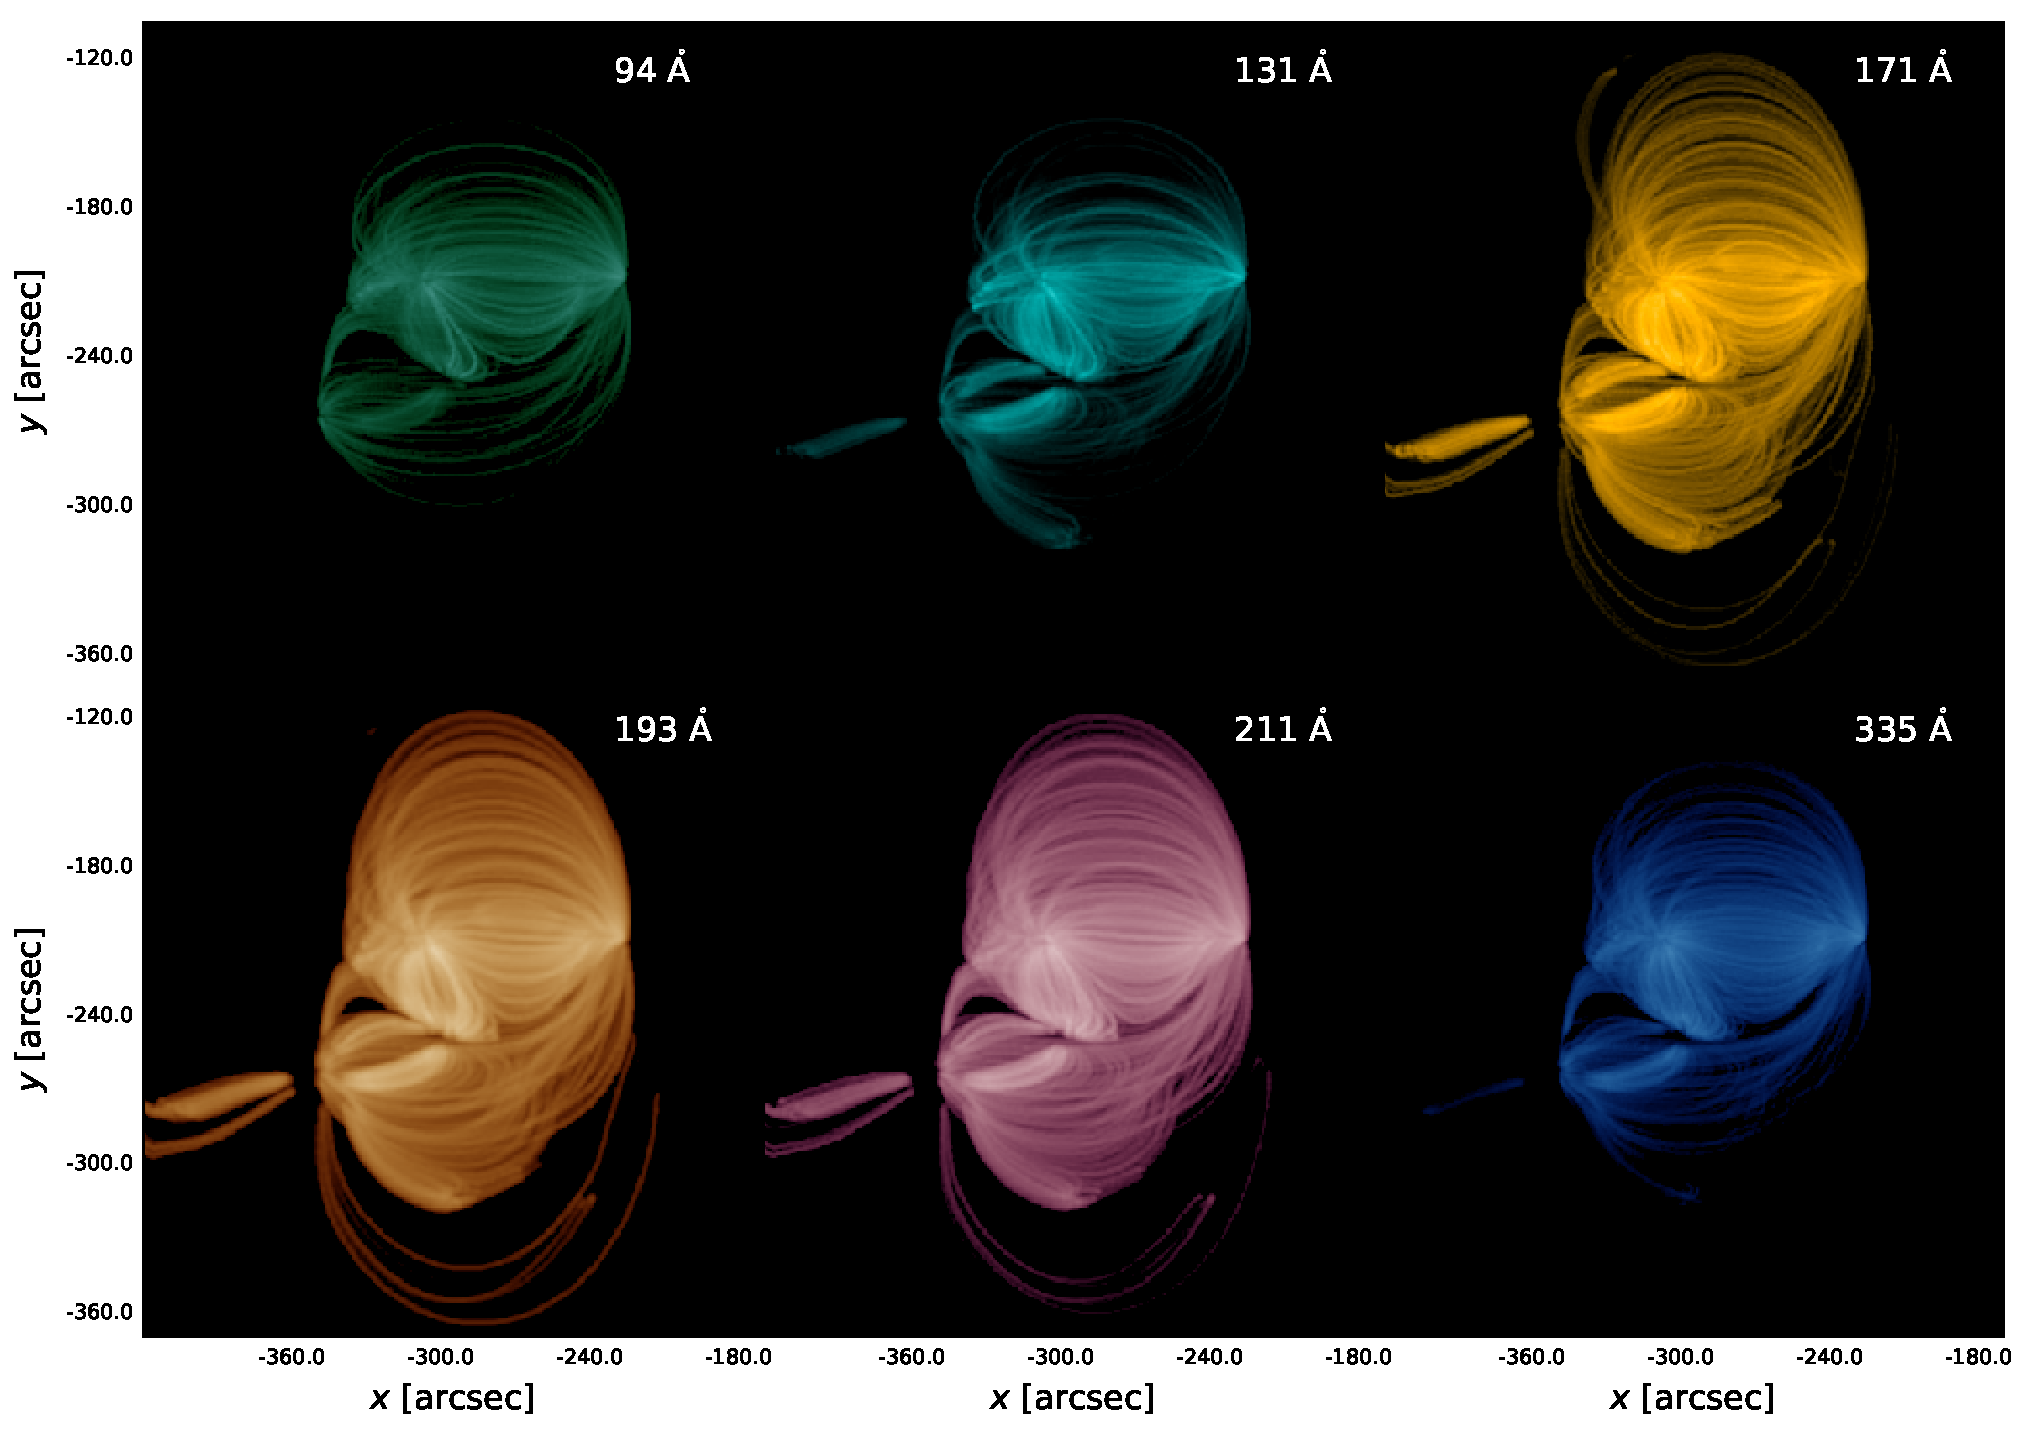
\includegraphics[width=\columnwidth]{figures/aia_intensities.pdf}
            \caption{AIA intensities} 
            \label{fig:synthesized_aia_maps}
            \centering
        \end{figure}
    \end{block}
    %
    %
  \end{column}
  %%
%%%%%%%%%%%%%%%%%%%%%%%%%%%%%%%%%%%%%%%%%%%%%%%%%
  %%second column
  \begin{column}{0.49\linewidth}
    % Heating model
    %% Explain heating models, energy distribution
    \begin{block}{Heating Models}
        \begin{columns}[T]
        \begin{column}{0.49\columnwidth}
            \begin{itemize}
            \item Nanoflare model of \citet{parker_nanoflares_1988}: corona heated by impulsive ($\ll\tau_{cool}$), low-energy ($\sim10^{24}$ erg) events produced by twisting, braiding of field lines
            \item Each strand heated independently by repeating triangular pulses of duration $\tau=200$ s; preferentially heat electrons 
            \item Use extrapolated field strength to estimate total energy input per strand as,
            \begin{equation*}
                E = (\epsilon B)^2/8\pi
            \end{equation*}
            \item $\epsilon=0.1$ is the stressing coefficient and $B$ is the average field strength per strand
            \item Event energies chosen from a power-law distribution with $\alpha=-2.5$ such that total energy constrained as above
            \item Choose four different average waiting times $\langle t_N\rangle=250,\,750,\,2500,\,5000$ s 
            \begin{itemize}
            \item Range from high-frequency heating (250 s) to low-frequency heating (5000 s)
            \item $t_{N,i}\propto E_i$ such that larger events require a longer ``winding time'', consistent with Parker nanoflare picture \citep[e.g.][]{cargill_active_2014,barnes_inference_2016-1}
            \end{itemize}
            \end{itemize}
        \end{column}
        \begin{column}{0.49\columnwidth}
            \begin{figure}
                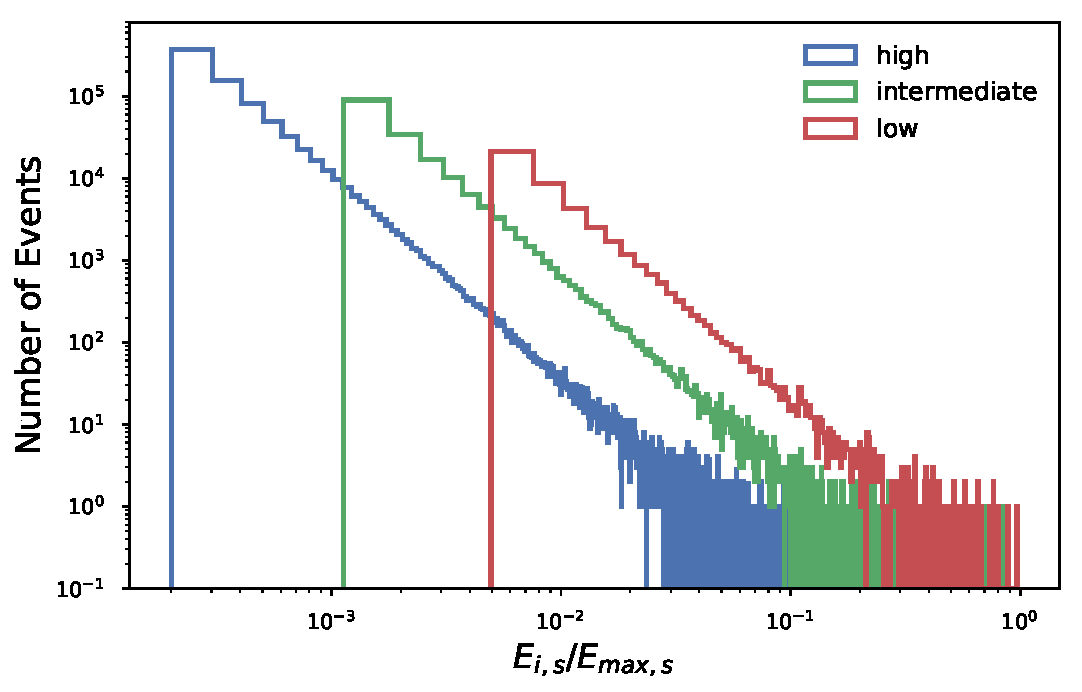
\includegraphics[width=\columnwidth]{figures/heating_rate_distributions.pdf}
                \caption{Energy distribution} 
                \label{fig:wait_times}
            \end{figure}
            \begin{figure}
                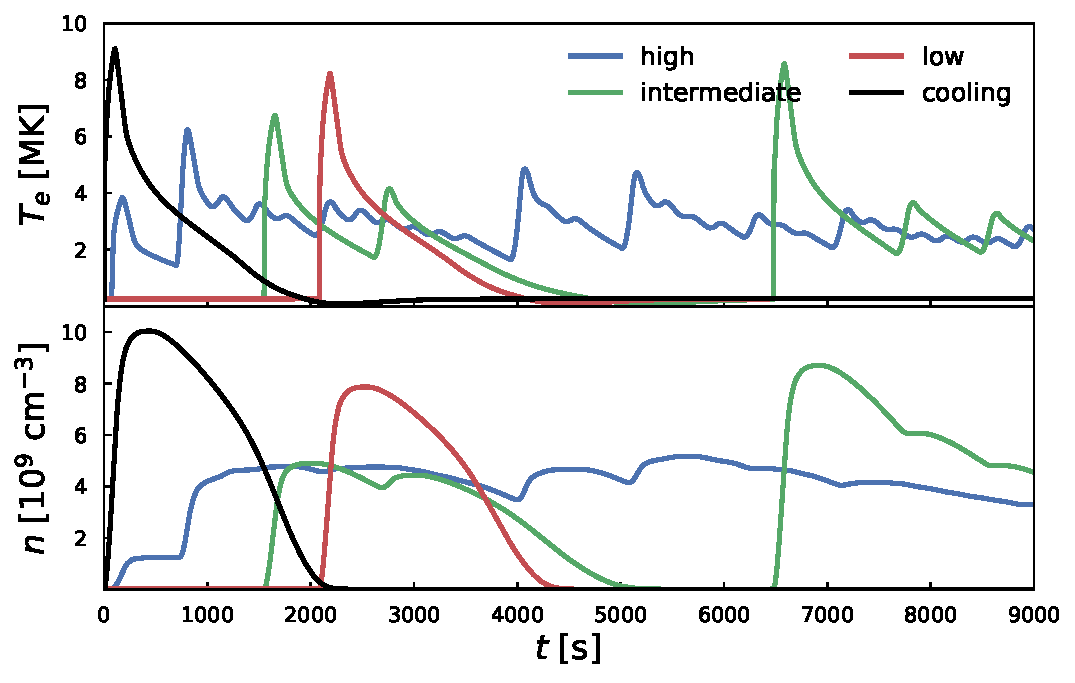
\includegraphics[width=\columnwidth]{figures/hydrodynamic_nT.pdf}
                \caption{Loop hydrodynamics} 
                \label{fig:hydrodynamics}
            \end{figure}
        \end{column}
        \end{columns}
    \end{block}
    % 
    % cross correlations
    \begin{block}{Cross-correlation of Channel Pairs}
        \begin{columns}[T]
            \begin{column}{0.49\columnwidth}
            \begin{figure}
                \subfigure{%
                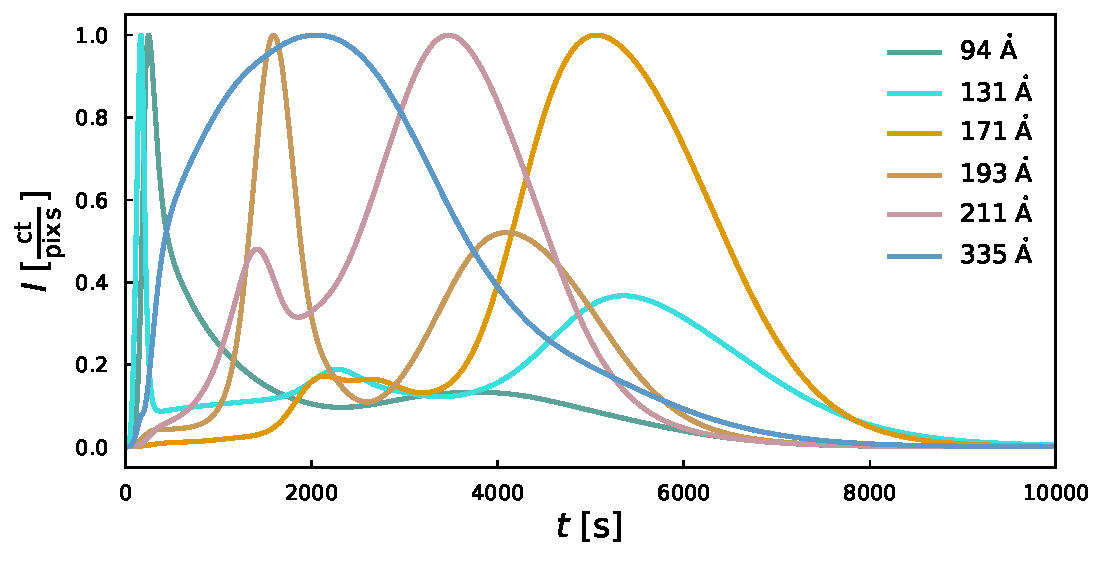
\includegraphics[width=\columnwidth]{figures/cooling_timeseries_1d.pdf}
                \label{fig:aia_lightcurves}}
                \subfigure{%
                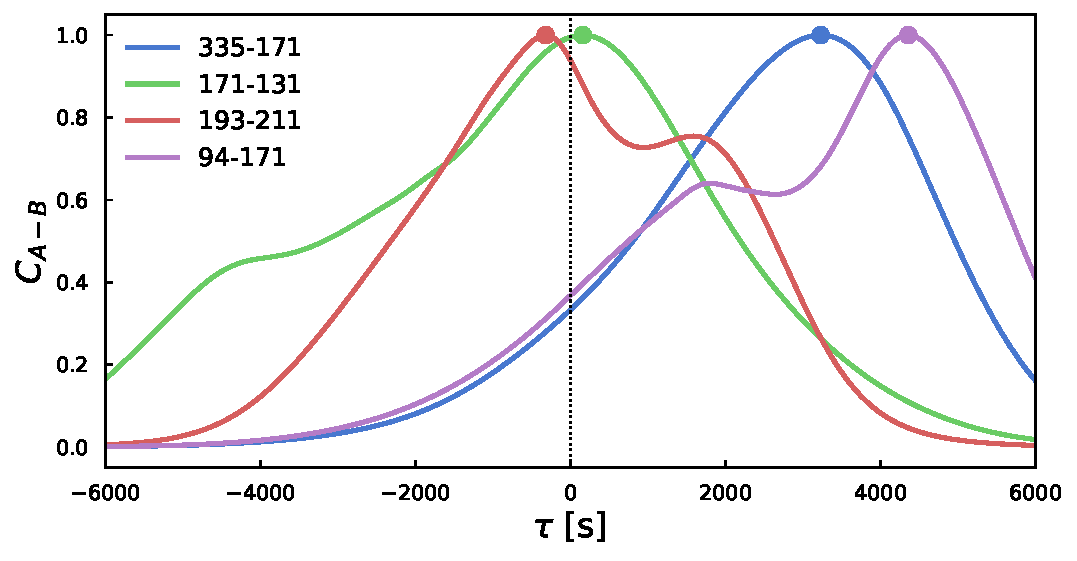
\includegraphics[width=\columnwidth]{figures/cooling_cross_correlations_1d.pdf}
                \label{fig:1d_correlations}}
                \caption{\textbf{Top:} Normalized timeseries for all of the AIA channels for the cooling-only case. Note that the intensity peaks in successively cooler channels as the loops cool from well above 10 MK to below 1 MK. This timeseries is extracted from a single-pixel in the center of the AR. \textbf{Bottom:} Normalized cross-correlation curves as a function offset for several different channel pairs. }
            \end{figure}
            \end{column}
            \begin{column}{0.49\columnwidth}
                \begin{itemize}
                    \item The cross-correlation, $C_{A,B}(\tau)$, between two timeseries $s_A(t)$ and $s_B(t)$, can be expressed as,
                    \begin{equation}
                        C_{A,B}(\tau) = \mathcal{F}^{-1}\{\mathcal{F}\{s_A(-t)\}\mathcal{F}\{s_B(t)\}\}
                    \end{equation}
                    where $\mathcal{F}$ is the Fourier transform and $\tau$ is the offset
                    \item Define the \alert{timelag} between two channels $A$ and $B$, $\tau^*_{A,B}$, as that offset which maximizes the cross-correlation,
                    \begin{equation}
                        \tau^*_{A,B} = \argmax_{\tau}C_{AB}(\tau)
                    \end{equation}
                    \item By convention, $\tau^*_{A,B}>0$ indicates that the peak in $s_A$ is followed by the peak in $s_B$
                    \item For a channel pair $A,B$ such that temperature of peak sensitivity of $A$ is greater than that of $B$, $\tau^*_{A,B}>0$ indicates that the plasma is \alert{cooling through} the instrument passbands of first channel $A$ and then channel $B$, e.g. the 335-171 pair shown in Fig. \ref{fig:1d_correlations}
                    \item Compute $C_{A,B}$ and $\tau^*_{A,B}$ in each pixel of the AR (see Fig. \ref{fig:timelag_maps})--understand cooling patterns for a given heating model and compare to observed $\tau^*_{A,B}$
                \end{itemize}
                \begin{figure}
                    \begin{columns}
                        \column{0.6\columnwidth}
                        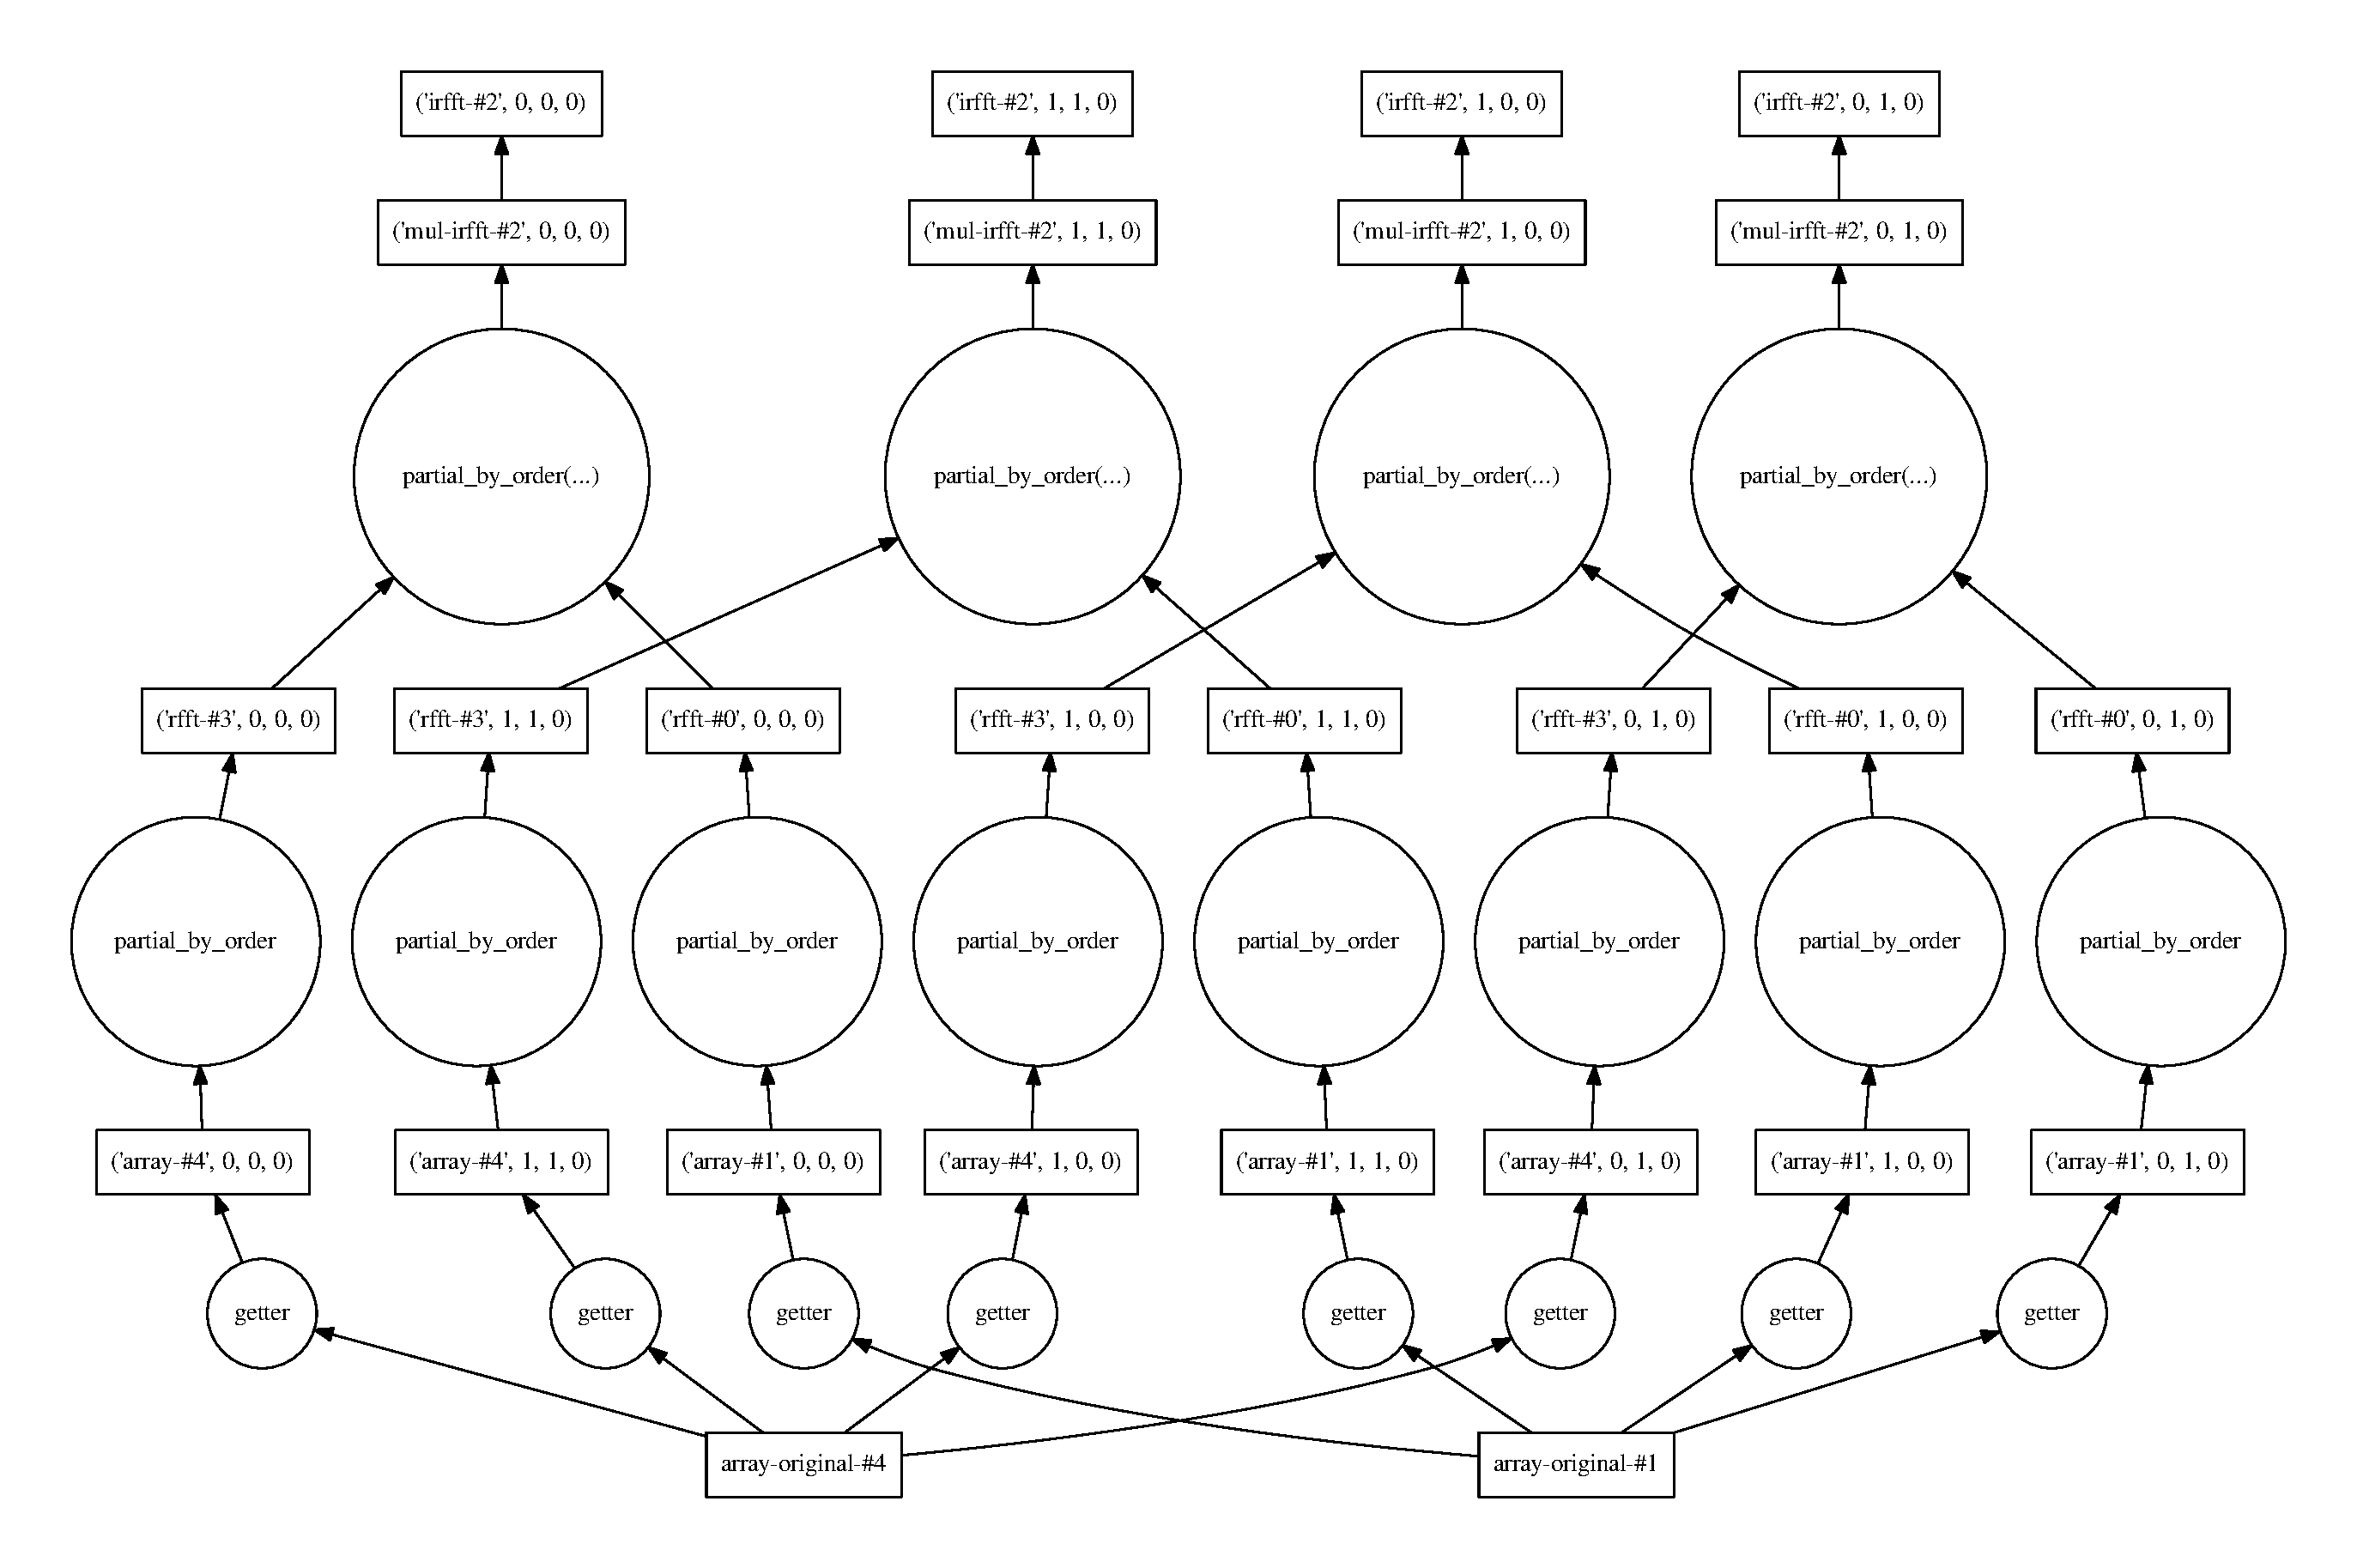
\includegraphics[width=\columnwidth]{figures/timelag_dag.pdf}
                        \column{0.35\columnwidth}
                        \caption{Example DAG for the cross-correlation calculation over the whole AR. Using the Dask Python library \citep{dask_development_team_dask:_2016} for distributed computation, this calculation can be efficiently scaled across many cores such that $\sim10^4$ timelags can be computed in a matter of a few minutes.}
                    \end{columns}
                    \label{fig:timelag_dask_dag}
                \end{figure}
            \end{column}
        \end{columns}
    \end{block}
    %
    % timelag maps
    %% maps of maximum timelags
    \begin{block}{Timelag Maps}
        \begin{figure}
            \subfigure{%
            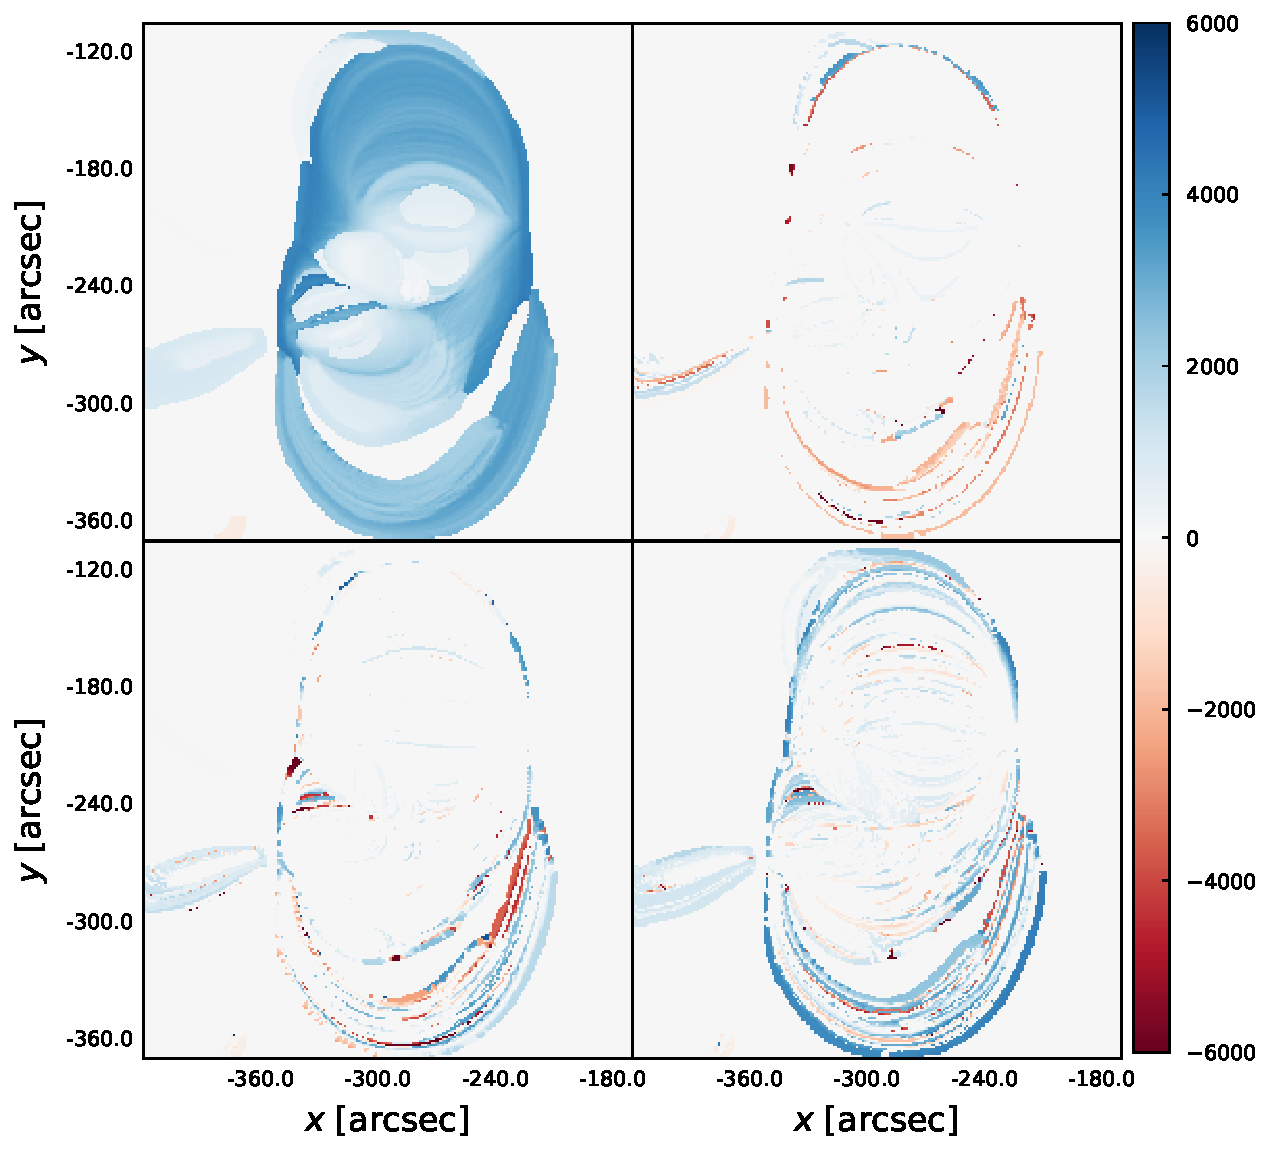
\includegraphics[width=0.54\columnwidth]{figures/timelag_maps_335_171.pdf}
            \label{fig:timelag_maps}}
            \subfigure{%
            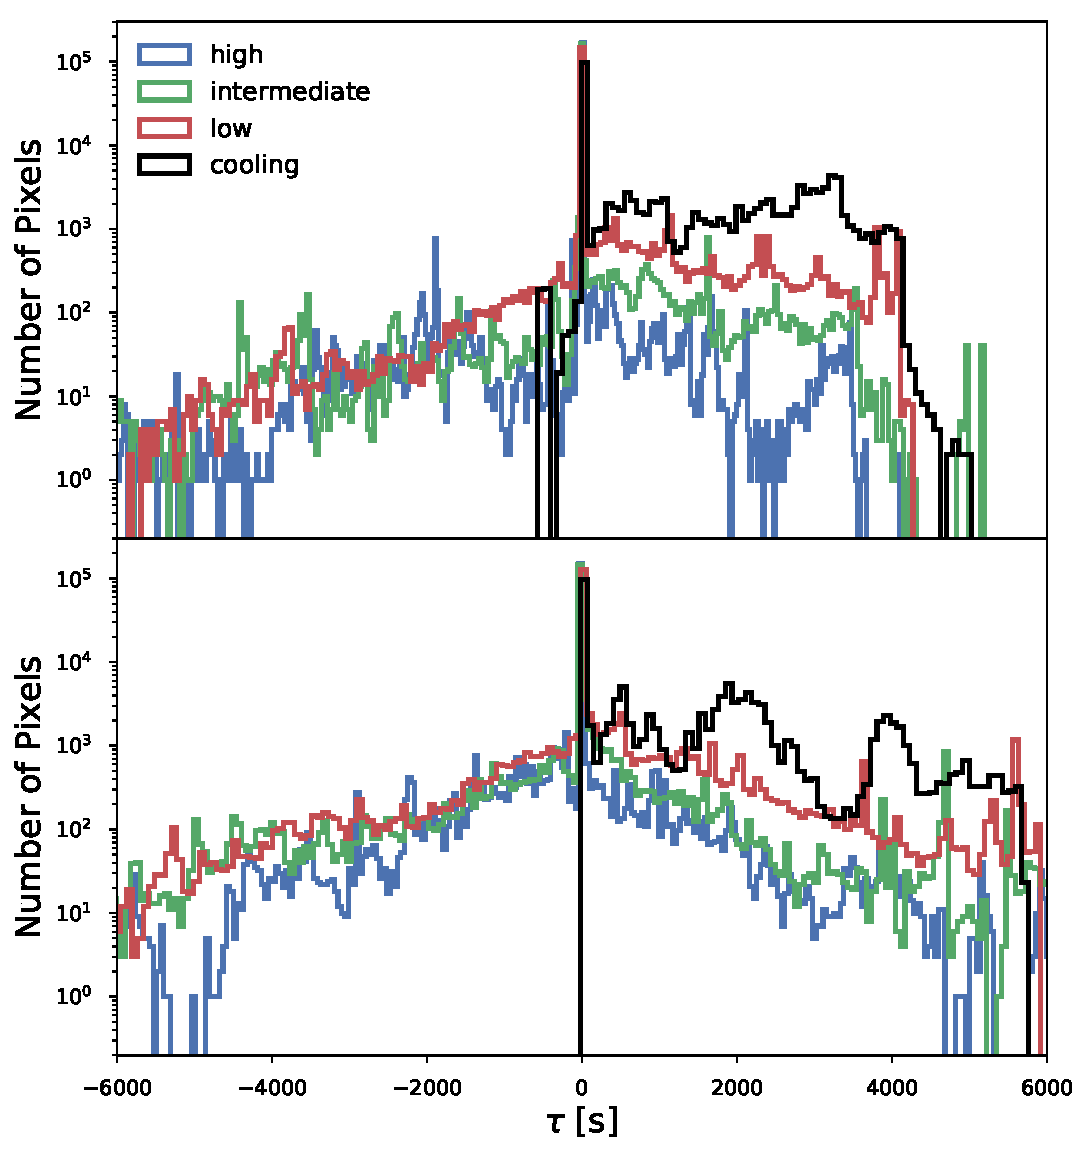
\includegraphics[width=0.45\columnwidth]{figures/timelag_histograms.pdf}
            \label{fig:timelag_histos}}
            \caption{caption goes here}
            \label{fig:timelags}
        \end{figure}
    \end{block}
    %
    %Conclusions
    \begin{block}{Conclusions}
      \begin{itemize}
        \item some Conclusions
        \item about the timelag results
        \item can go here
      \end{itemize}
    \end{block}
    %
    %references
    \begin{block}{References}
      \scriptsize
      \begin{multicols}{2}
        \bibliographystyle{../apj.bst}
        \bibliography{references.bib}
      \end{multicols}
    \end{block}
  \end{column}
  \end{columns}
\end{frame}
\end{document}
